\chapter{Trích xuất tri thức từ dữ liệu}

\section{Tổng quan quy trình trích xuất}

Mục tiêu của quy trình trích xuất là chuyển đổi dữ liệu phi cấu trúc thành các mảnh tri thức ban đầu có thể tổ chức trong đồ thị. Ở giai đoạn này, hệ thống chưa tạo ra đồ thị tri thức cuối cùng, mà tập trung nhận diện các đối tượng quan trọng, các quan hệ có căn cứ trong tài liệu và thông tin nguồn để phục vụ kiểm tra ở các bước sau.

Ở mức tổng quan, quy trình trích xuất gồm bốn nhóm chức năng chính. Nhóm thứ nhất chuẩn bị và tổ chức dữ liệu đầu vào để nội dung được xử lý theo các đơn vị rõ ràng. Nhóm thứ hai xác định ngữ cảnh và các quy tắc biểu diễn tri thức, giúp kết quả trích xuất thống nhất hơn giữa nhiều tài liệu. Nhóm thứ ba nhận diện thực thể, thuộc tính và quan hệ xuất hiện trong văn bản. Nhóm thứ tư kiểm tra, làm sạch và lưu lại kết quả cùng thông tin truy vết nguồn gốc.

Đầu ra của quy trình trích xuất là một đồ thị thô, đóng vai trò dữ liệu trung gian cho toàn bộ quy trình xây dựng đồ thị tri thức. Đồ thị thô này vẫn có thể chứa thực thể trùng lặp, đồng tham chiếu, quan hệ chưa nhất quán hoặc thông tin cần được kiểm tra thêm. Vì vậy, kết quả sau trích xuất sẽ được chuyển sang bước xử lý đồng tham chiếu thực thể ở Chương~5 để giảm phân mảnh và nâng cao tính nhất quán của đồ thị. Quy trình tổng quan được minh họa trong Hình~\ref{fig:extraction-pipeline}.

\begin{figure}[H]
    \centering
    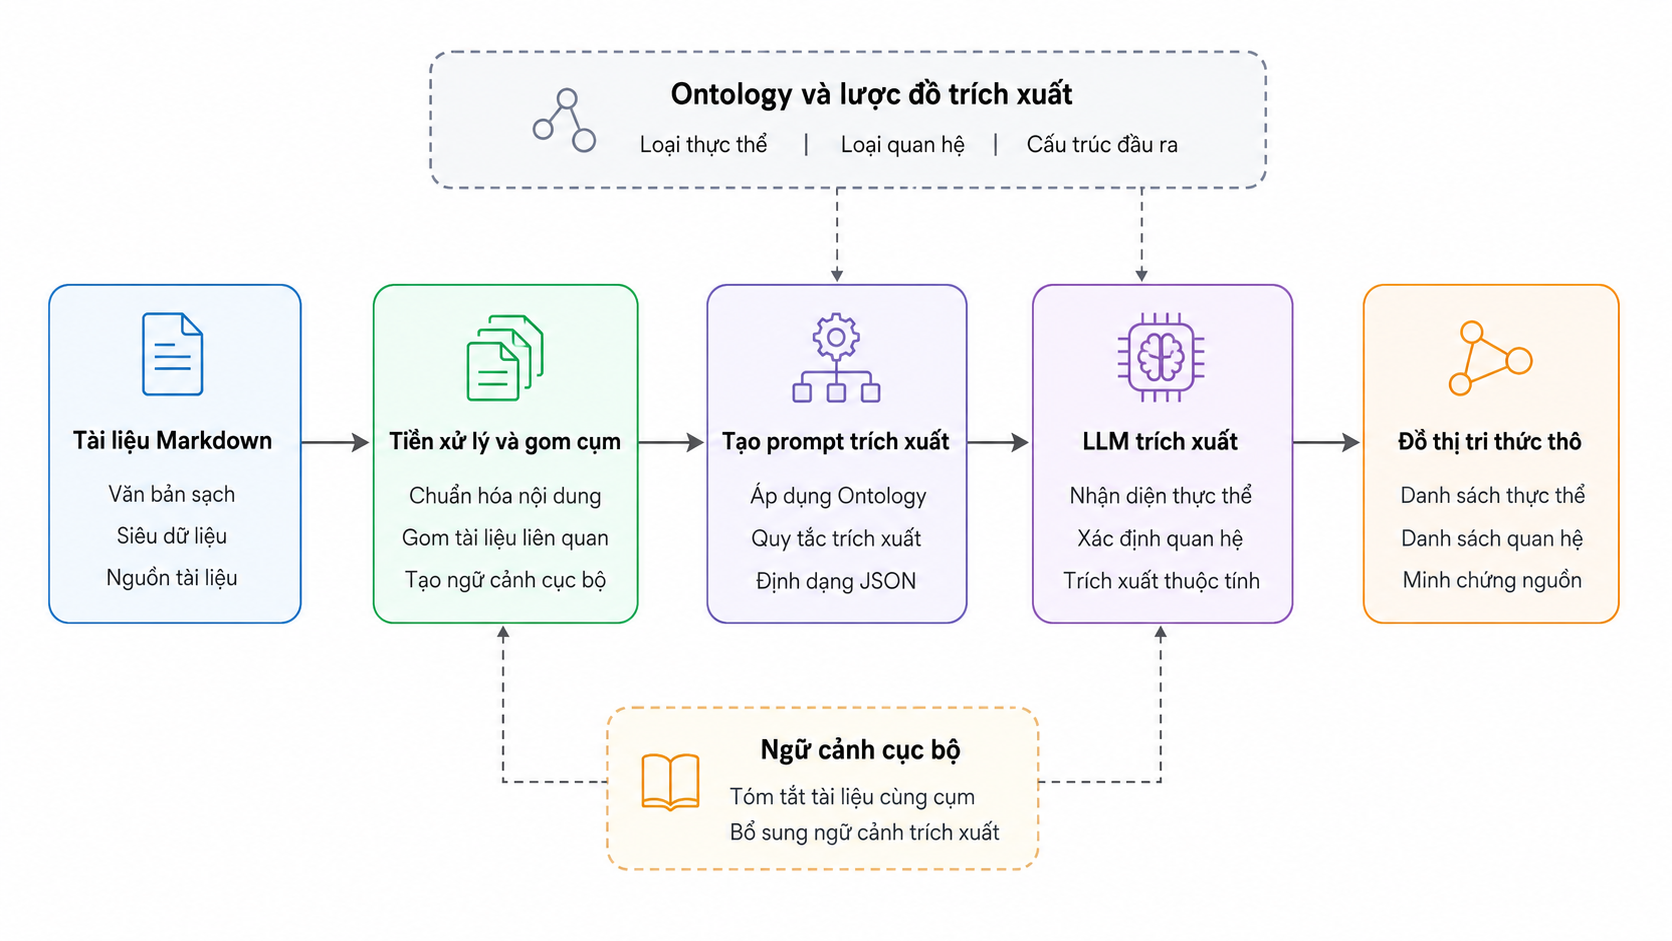
\includegraphics[width=\textwidth]{image/generated/chapter4/extraction-pipeline.png}
    \caption{Quy trình trích xuất tri thức từ dữ liệu}
    \label{fig:extraction-pipeline}
\end{figure}

\section{Xử lý và phân đoạn dữ liệu}

Dữ liệu đầu vào của khóa luận được thu thập tự động từ các trang tin tức công khai của Trường Đại học Công nghệ. Dữ liệu sau khi thu thập thường chưa ở trạng thái phù hợp để trích xuất tri thức trực tiếp, vì nội dung trên trang tin tức có thể chứa nhiều thành phần không cần thiết như thanh điều hướng, chân trang, liên kết lặp lại hoặc các đoạn văn bản không mang nhiều thông tin. Do đó, bước xử lý dữ liệu có nhiệm vụ làm sạch nội dung và đưa dữ liệu về một dạng biểu diễn thống nhất.

Trong khóa luận này, dữ liệu sau khi xử lý được chuẩn hóa về dạng Markdown. Dạng biểu diễn này giữ lại được cấu trúc cơ bản của tài liệu như tiêu đề, đoạn văn, danh sách và liên kết, đồng thời loại bỏ bớt các yếu tố trình bày không cần thiết của trang tin tức. Việc chuẩn hóa dữ liệu giúp các bước sau làm việc với một đầu vào nhất quán hơn, thay vì phải xử lý trực tiếp nhiều dạng nội dung khác nhau từ các trang tin tức.

Một vấn đề quan trọng trong giai đoạn này là lượng dữ liệu đầu vào ảnh hưởng trực tiếp đến chất lượng kết quả trích xuất. Mô hình ngôn ngữ lớn chỉ có thể xử lý một lượng ngữ cảnh hữu hạn trong mỗi lần suy luận. Nếu đưa một tài liệu quá dài hoặc quá nhiều tài liệu vào cùng một lần xử lý, nội dung có thể vượt quá giới hạn ngữ cảnh của mô hình, làm mất thông tin quan trọng hoặc khiến kết quả đầu ra thiếu ổn định. Ngược lại, nếu chia dữ liệu quá nhỏ, các đoạn văn bản có thể mất ngữ cảnh cần thiết để nhận diện đúng thực thể và quan hệ.

Vì vậy, dữ liệu cần được phân đoạn trước khi đưa vào bước trích xuất tri thức. Phân đoạn dữ liệu, hay chunking, là quá trình chia nội dung thành các đơn vị xử lý nhỏ hơn nhưng vẫn cố gắng giữ được ý nghĩa tương đối đầy đủ của từng đoạn. Cách tổ chức này giúp hạn chế tình trạng tràn ngữ cảnh của mô hình ngôn ngữ lớn, đồng thời tạo điều kiện để hệ thống kiểm soát tốt hơn chất lượng đầu vào cho từng lần trích xuất.

Trong quá trình xử lý, mỗi tài liệu hoặc phân đoạn dữ liệu được gắn với thông tin nguồn tương ứng. Thông tin này cho phép truy ngược kết quả trích xuất về tài liệu ban đầu, hỗ trợ kiểm tra bằng chứng và sửa lỗi khi cần thiết. Như vậy, bước xử lý và phân đoạn dữ liệu không chỉ chuẩn bị đầu vào cho mô hình, mà còn đặt nền tảng cho tính minh bạch và khả năng kiểm chứng của đồ thị tri thức ở các bước sau.

\section{Gom nhóm dữ liệu và duy trì ngữ cảnh}

Sau khi dữ liệu được xử lý và phân đoạn, mỗi đoạn dữ liệu (chunk) vẫn chỉ chứa một phần ngữ cảnh của toàn bộ nguồn dữ liệu. Một chủ đề có thể được phân tán trên nhiều trang khác nhau, trong khi cùng một thực thể có thể xuất hiện dưới nhiều cách gọi như tên đầy đủ, tên viết tắt hoặc tên theo ngữ cảnh. Nếu từng đoạn dữ liệu được đưa vào trích xuất một cách hoàn toàn độc lập, các phiên trích xuất dễ tạo ra những mảnh tri thức rời rạc, thiếu liên kết với nhau. Vì vậy, bước gom nhóm dữ liệu được sử dụng để đưa các đoạn có khả năng liên quan vào cùng một nhóm, dựa trên nguyên tắc tương đồng nội dung (content similarity).

Mục tiêu của việc gom nhóm trong giai đoạn này không phải là giải quyết triệt để bài toán đồng tham chiếu thực thể. Việc hợp nhất thực thể ở phạm vi toàn cục sẽ được trình bày ở Chương~5. Ở đây, bước gom nhóm đóng vai trò giảm bớt sự rời rạc ban đầu của dữ liệu, giúp các đoạn cùng chủ đề hoặc cùng nhắc đến một nhóm thực thể được xử lý gần nhau hơn. Có thể xem kết quả của bước này là các nhóm đoạn liên quan (related chunks), tạo điều kiện để hệ thống tái sử dụng thông tin đã trích xuất trước đó trong phạm vi nhóm, thay vì xử lý từng đoạn như những đơn vị hoàn toàn tách biệt.

Cách thực hiện gom nhóm bắt đầu từ việc biểu diễn mỗi đoạn bằng một tập từ khóa đại diện. Trong cài đặt của khóa luận, các từ khóa này được lấy từ tên tệp hoặc đường dẫn sau khi đã chuẩn hóa, sau đó loại bỏ những từ ít mang ý nghĩa. Hệ thống tính độ tương đồng Jaccard giữa các tập từ khóa để ước lượng mức độ gần nhau giữa hai đoạn. Nếu độ tương đồng vượt qua một ngưỡng định trước, các đoạn được đưa vào cùng một nhóm; nếu không, hệ thống tạo nhóm mới. Đây là một cách cài đặt cụ thể của nguyên tắc gom nhóm theo tương đồng nội dung, phù hợp với dữ liệu thu thập từ trang tin tức vì tên trang và đường dẫn thường phản ánh chủ đề chính của nội dung.

Sau khi có các nhóm dữ liệu, hệ thống cần duy trì ngữ cảnh cục bộ (local context) bên trong từng nhóm. Với mỗi nhóm, local context ban đầu rỗng. Sau khi một đoạn được trích xuất thành công, hệ thống lưu lại các thực thể quan trọng, tên gọi thay thế và một số quan hệ hoặc sự kiện vừa nhận diện được. Phần ngữ cảnh này được cập nhật dần theo kiểu tóm tắt cuốn chiếu (rolling summary), rồi được đưa vào đầu vào của mô hình khi xử lý đoạn tiếp theo trong cùng nhóm. Nhờ đó, mô hình có thêm căn cứ để nhận diện lại các thực thể đã xuất hiện trước đó và giảm sự thiếu nhất quán giữa các lần trích xuất.

Nhờ local context, các phiên trích xuất trong cùng một nhóm không còn hoàn toàn độc lập. Ví dụ, nếu một đoạn trước đã ghi nhận Trường Đại học Công nghệ, Đại học Công nghệ và UET là các cách gọi liên quan đến cùng một đơn vị, đoạn sau trong cùng nhóm có thêm tín hiệu để sử dụng tên gọi nhất quán hơn. Cơ chế này giúp giảm một phần sự phân mảnh ngay từ giai đoạn trích xuất, đồng thời tạo đầu vào tốt hơn cho bước xử lý đồng tham chiếu thực thể ở chương tiếp theo.

\section{Xây dựng prompt trích xuất tri thức}

Prompt là phần chỉ dẫn đầu vào được gửi cho mô hình ngôn ngữ lớn để mô tả nhiệm vụ, cung cấp ngữ cảnh, đặt ra ràng buộc và quy định dạng kết quả cần sinh. Trong bài toán trích xuất tri thức, prompt không chỉ nêu yêu cầu mô hình đọc văn bản, mà còn chỉ rõ mô hình cần nhận diện loại thực thể nào, quan hệ nào được phép tạo, thông tin bằng chứng nào cần giữ lại và kết quả phải được biểu diễn theo cấu trúc nào.

Trong trích xuất tri thức bằng mô hình ngôn ngữ lớn, prompt có ảnh hưởng trực tiếp đến chất lượng và hình dạng của đồ thị được sinh ra. Cùng một đoạn văn bản có thể tạo ra các kết quả khác nhau nếu mô hình không được hướng dẫn rõ về phạm vi miền tri thức, kiểu thực thể cần nhận diện, kiểu quan hệ cần ưu tiên và cấu trúc đầu ra mong muốn. Vì vậy, prompt trong khóa luận không chỉ là một câu lệnh yêu cầu trích xuất thông tin, mà là cơ chế chuyển ontology và schema thành các chỉ dẫn cụ thể để kiểm soát quá trình sinh tri thức.

Ontology và schema là hai thành phần nền tảng trong quá trình xây dựng prompt. Ontology giúp xác định các khái niệm thuộc miền dữ liệu cần quan tâm, chẳng hạn trường đại học, đơn vị trực thuộc, chương trình đào tạo, cán bộ, sự kiện, văn bản hoặc địa điểm. Schema quy định cách các khái niệm đó được biểu diễn trong đồ thị, bao gồm kiểu thực thể, kiểu quan hệ, thuộc tính cần lưu và yêu cầu về bằng chứng. Theo Noy và McGuinness, xây dựng ontology cần bắt đầu từ việc xác định miền và phạm vi, liệt kê thuật ngữ quan trọng, xác định lớp, thuộc tính và các ràng buộc liên quan \cite{noy2001ontology}. Các nguyên tắc này được sử dụng trong khóa luận để xác định những loại tri thức cần trích xuất từ dữ liệu của Trường Đại học Công nghệ.

Qua quá trình nghiên cứu và thực nghiệm, có thể khái quát hai dạng cấu trúc prompt chính cho bài toán trích xuất tri thức. Dạng thứ nhất là prompt không kiểm soát kiểu thực thể và quan hệ, tức mô hình được để tự do quyết định đối tượng nào nên trở thành thực thể và quan hệ nào nên được sinh ra. Cách này có ưu điểm là linh hoạt, nhưng dễ tạo ra nhiều nhãn thực thể khác nhau cho cùng một loại đối tượng, nhiều tên quan hệ có nghĩa gần nhau nhưng cách viết khác nhau, và các mảnh đồ thị khó hợp nhất ở các bước sau.

Dạng thứ hai là prompt có kiểm soát, trong đó kiểu thực thể, định hướng quan hệ và quy tắc biểu diễn được xác định trước dựa trên ontology và schema. Cách này giúp đầu ra của mô hình ổn định hơn, dễ kiểm tra hơn và phù hợp hơn với mục tiêu xây dựng đồ thị tri thức có cấu trúc. Các nghiên cứu gần đây về xây dựng đồ thị tri thức bằng mô hình ngôn ngữ lớn cũng nhấn mạnh rằng trích xuất cần đi kèm với bước định nghĩa và chuẩn hóa tri thức, thay vì để mô hình sinh kết quả hoàn toàn tự do \cite{zhang2024extract}. Vì vậy, khóa luận lựa chọn hướng prompt có kiểm soát.

Cụ thể, khóa luận kiểm soát chặt các kiểu thực thể được phép tạo ra bằng một tập nhãn thực thể định nghĩa trước. Mô hình chỉ được tạo thực thể thuộc các kiểu nằm trong tập này, nhờ đó hạn chế tình trạng sinh nhãn tùy ý hoặc tạo nút cho các khái niệm quá chung. Đối với quan hệ, khóa luận sử dụng cách kiểm soát mềm hơn: prompt đưa ra các tên quan hệ được ưu tiên và các quy tắc sinh quan hệ để định hướng mô hình. Cách thiết kế này giữ được khả năng biểu diễn các quan hệ đa dạng trong văn bản tự nhiên, nhưng vẫn hạn chế các quan hệ dài, mơ hồ hoặc khó tái sử dụng. Trong những hệ thống yêu cầu quản lý chặt chẽ hơn, tập quan hệ cũng có thể được định nghĩa đóng hoàn toàn tương tự như tập kiểu thực thể.

Cấu trúc tổng thể của prompt trích xuất tri thức trong khóa luận gồm các phần chính sau. Phần mở đầu là hướng dẫn nhiệm vụ, nêu vai trò của mô hình và yêu cầu trích xuất thực thể, thuộc tính, quan hệ từ văn bản dựa trên bằng chứng. \texttt{ENTITY LABELS} định nghĩa tập kiểu thực thể được phép tạo ra; phần này thể hiện trực tiếp ảnh hưởng của ontology đối với phạm vi tri thức được trích xuất. \texttt{ENTITY RULES} quy định cách tạo thực thể, cách chọn tên chuẩn, cách xử lý tên viết tắt hoặc tên thay thế, và khi nào không nên tạo một thực thể mới. \texttt{PREFERRED RELATIONSHIP NAMES} cung cấp các tên quan hệ nên được ưu tiên tái sử dụng khi văn bản có liên kết phù hợp. \texttt{RELATIONSHIP RULES} quy định khi nào được tạo quan hệ, cách đặt tên quan hệ, yêu cầu quan hệ phải có căn cứ trong văn bản và cách mô tả liên kết giữa hai thực thể. \texttt{OUTPUT SCHEMA} định nghĩa cấu trúc đầu ra để kết quả có thể được kiểm tra, lưu trữ và chuyển sang các bước xử lý sau. Cuối cùng là phần văn bản đầu vào, tức đoạn dữ liệu đã được xử lý và đưa vào prompt để mô hình thực hiện trích xuất.

Hình~\ref{fig:kg-prompt} minh họa cấu trúc tổng thể của prompt trích xuất tri thức. Hình này cho thấy prompt được xây dựng từ nhiều lớp: hướng dẫn nhiệm vụ, ontology, schema, quy tắc thực thể, quy tắc quan hệ, cấu trúc đầu ra và văn bản đầu vào. Sự kết hợp này giúp quá trình trích xuất không chỉ dựa vào khả năng sinh ngôn ngữ của mô hình, mà còn được định hướng bởi các quyết định thiết kế tri thức của khóa luận.

\begin{figure}[H]
    \centering
    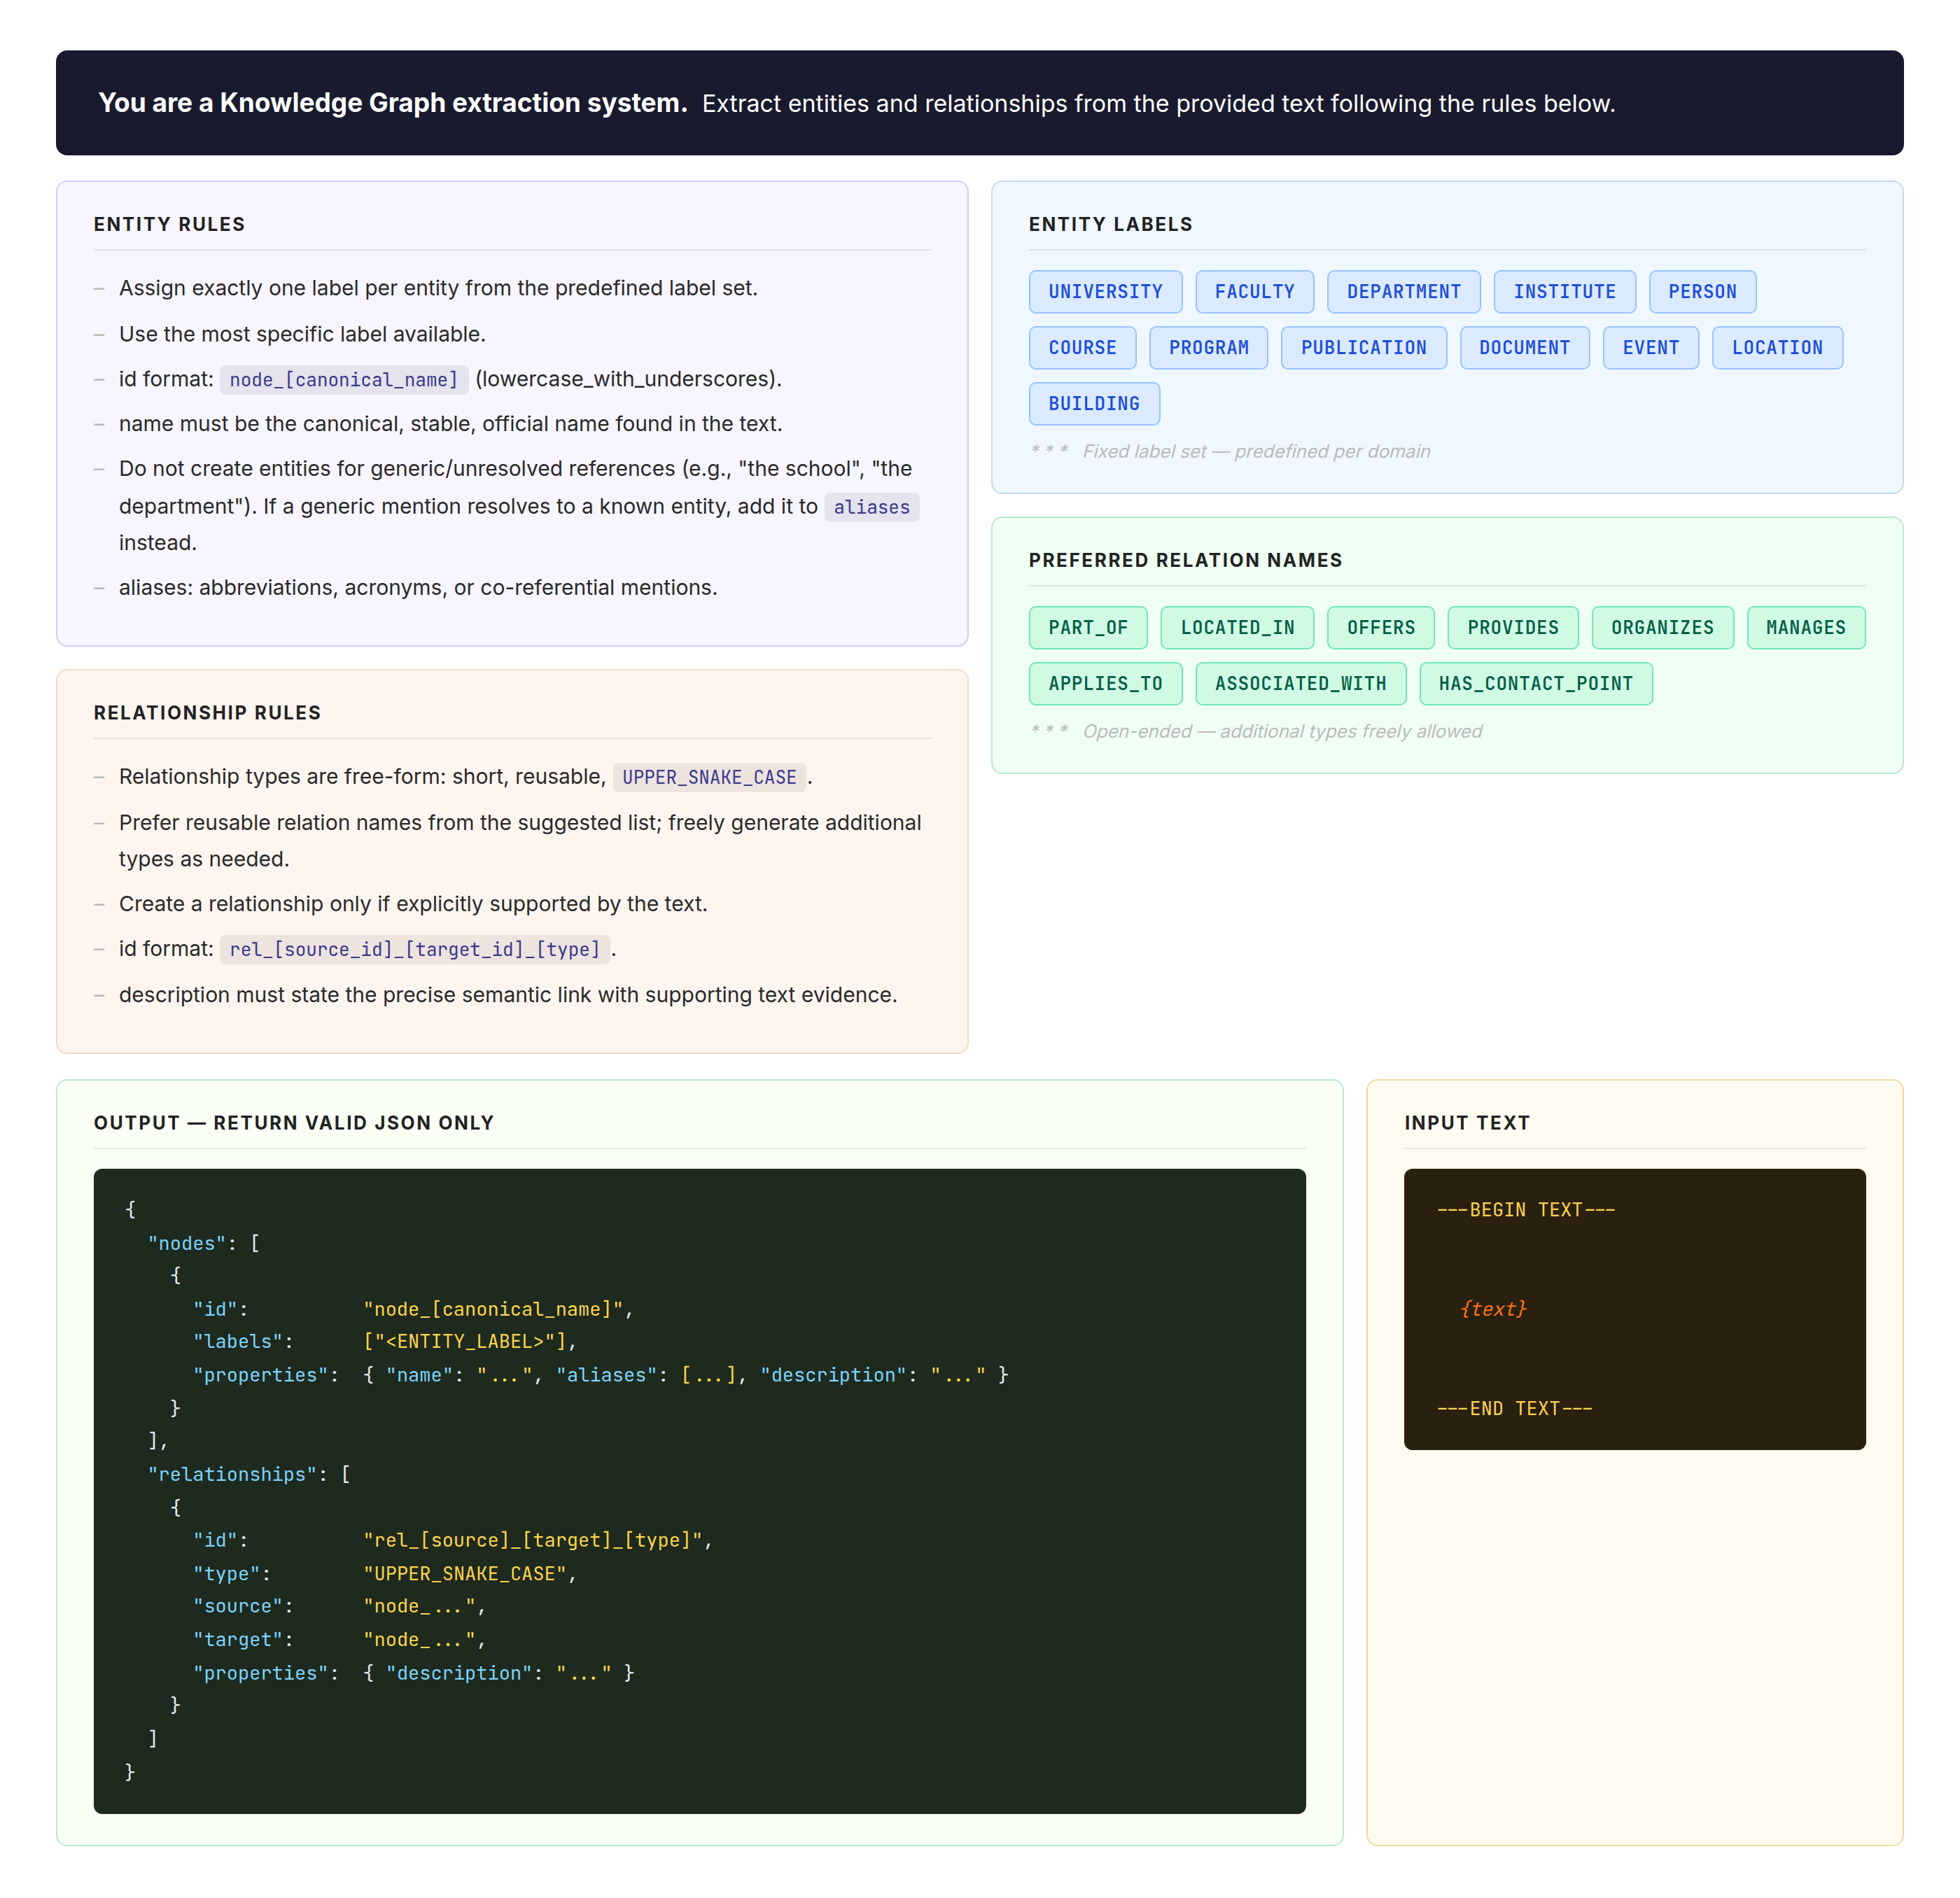
\includegraphics[width=\textwidth]{image/generated/chapter4/kg_prompt.png}
    \caption{Cấu trúc prompt trích xuất tri thức}
    \label{fig:kg-prompt}
\end{figure}

\section{Kết quả của trích xuất tri thức}

Sau khi áp dụng quy trình trích xuất trên tập dữ liệu đã thu thập, kết quả đầu ra là các mảnh đồ thị tri thức ở dạng JSON. Trong lần chạy hiện tại, quy trình xử lý 1.003 đơn vị dữ liệu và sinh ra 12.081 thực thể thô cùng 12.321 quan hệ thô. Các con số này phản ánh kết quả ngay sau giai đoạn trích xuất, trước khi thực hiện xử lý đồng tham chiếu thực thể và chuẩn hóa đồ thị ở Chương~5.

Kết quả sau trích xuất chưa phải là một đồ thị tri thức hoàn chỉnh. Do mỗi đoạn dữ liệu chỉ chứa một phần ngữ cảnh, đầu ra thường có dạng các đồ thị nhỏ rời rạc, mỗi đồ thị gắn với một tài liệu hoặc một phân đoạn cụ thể. Bên cạnh đó, cùng một đối tượng trong thực tế có thể được tạo thành nhiều thực thể khác nhau do khác biệt về tên đầy đủ, tên viết tắt, tên tiếng Anh hoặc cách gọi theo ngữ cảnh. Ví dụ, Trường Đại học Công nghệ có thể xuất hiện dưới các cách gọi như Trường ĐHCN, Đại học Công nghệ hoặc UET. Đặc điểm này cho thấy bước xử lý đồng tham chiếu thực thể là cần thiết để nối các mảnh đồ thị nhỏ thành một nguồn tri thức nhất quán hơn.

Ví dụ JSON - kết quả trích xuất. Trong ví dụ này, phần \texttt{nodes} chứa các thực thể được nhận diện từ văn bản, còn phần \texttt{relationships} chứa quan hệ giữa các thực thể đó. Các thuộc tính như \texttt{chunk\_id} và \texttt{description} giúp giữ lại liên kết với đoạn dữ liệu nguồn và bằng chứng mô tả.

\begin{jsonbox}
\{
  "nodes": [
    \{
      "id": "node\_uet",
      "labels": ["UNIVERSITY"],
      "properties": \{
        "name": "Đại học Công nghệ",
        "aliases": ["UET"],
        "chunk\_id": ["c1"],
        "description": ["Trường thành viên của ĐHQGHN."]
      \}
    \},
    \{
      "id": "node\_vnu",
      "labels": ["SYSTEM"],
      "properties": \{
        "name": "Đại học Quốc gia Hà Nội",
        "aliases": ["VNU"],
        "chunk\_id": ["c1"],
        "description": ["Trung tâm đại học lớn tại Việt Nam."]
      \}
    \}
  ],
  "relationships": [
    \{
      "id": "rel\_uet\_vnu\_MEMBER\_OF",
      "type": "MEMBER\_OF",
      "source": "node\_uet",
      "target": "node\_vnu",
      "properties": \{
        "chunk\_id": ["c1"],
        "description": ["UET trực thuộc VNU."]
      \}
    \}
  ]
\}
\end{jsonbox}

Đối với một thực thể trong \texttt{nodes}, trường \texttt{id} là định danh cục bộ của thực thể trong kết quả trích xuất. Trường \texttt{labels} cho biết kiểu thực thể, chẳng hạn trường đại học hoặc cá nhân. Phần \texttt{properties} lưu các thông tin mô tả của thực thể. Trong đó, \texttt{name} là tên chuẩn được chọn cho thực thể, \texttt{aliases} lưu các tên gọi thay thế hoặc tên viết tắt, \texttt{chunk\_id} cho biết đoạn dữ liệu nguồn, và \texttt{description} mô tả ngắn gọn bằng chứng hoặc thông tin chính được trích xuất từ văn bản.

Đối với một quan hệ trong \texttt{relationships}, trường \texttt{id} là định danh của quan hệ, trường \texttt{type} biểu diễn kiểu quan hệ, còn \texttt{source} và \texttt{target} lần lượt chỉ định hai thực thể ở hai đầu quan hệ. Các trường trong \texttt{properties} của quan hệ có vai trò tương tự như ở thực thể: lưu đoạn dữ liệu nguồn và phần mô tả giải thích vì sao quan hệ đó được tạo ra. Nhờ các trường này, mỗi thực thể và quan hệ trong đồ thị thô đều có thể được truy vết về nguồn dữ liệu ban đầu, hỗ trợ kiểm chứng, đánh giá chất lượng và sửa lỗi ở các bước sau.

Mặc dù prompt đã được kiểm soát bằng ontology và schema, trích xuất trực tiếp bằng mô hình ngôn ngữ lớn vẫn không thể tạo ngay một đồ thị tri thức hoàn chỉnh. Mô hình có thể bỏ sót thực thể hoặc quan hệ quan trọng khi thông tin được diễn đạt gián tiếp, có thể sinh quan hệ chưa đủ căn cứ nếu văn bản mơ hồ, hoặc tạo ra nhiều nút khác nhau cho cùng một đối tượng trong thực tế. Các nghiên cứu về tạo đồ thị tri thức bằng mô hình ngôn ngữ lớn cũng chỉ ra rằng sai lệch và suy diễn quá mức vẫn là rủi ro cần được kiểm soát khi mở rộng quy trình sinh tri thức \cite{parovic2025generating}.

Đối với dữ liệu tiếng Việt của Trường Đại học Công nghệ, vấn đề này càng rõ hơn do sự đa dạng của tên riêng, tên viết tắt và cách gọi không chính thức. Một đơn vị có thể được nhắc đến bằng tên đầy đủ, tên rút gọn, tên tiếng Anh hoặc chỉ bằng chức năng trong từng ngữ cảnh cụ thể. Nếu các biến thể này không được hợp nhất, đồ thị tri thức sẽ bị phân mảnh: quan hệ liên quan đến cùng một đối tượng bị chia ra nhiều nút, làm giảm khả năng truy vấn, tổng hợp và trả lời câu hỏi. Ngược lại, nếu hợp nhất sai các thực thể khác nhau, đồ thị có thể chứa các quan hệ không đúng.

Vì vậy, Chương~5 giữ vai trò then chốt trong toàn bộ quy trình xây dựng đồ thị tri thức. Chương này không chỉ là bước xử lý bổ sung sau trích xuất, mà là bước chuyển từ tập mảnh đồ thị thô sang một đồ thị tri thức có chất lượng tốt hơn. Thông qua việc phát hiện các thực thể đồng tham chiếu, chọn thực thể chuẩn, hợp nhất tên gọi thay thế và cập nhật lại các quan hệ, quy trình xử lý đồng tham chiếu thực thể giúp giảm phân mảnh, tăng tính nhất quán và tạo nền tảng đáng tin cậy hơn cho ứng dụng hỏi đáp ở các chương sau.
